\pdfoutput=1

\documentclass[11pt]{article}

\usepackage{ACL2023}

\usepackage{times}
\usepackage{latexsym}

\usepackage[T1]{fontenc}

\usepackage[utf8]{inputenc}

\usepackage{microtype}
\usepackage{graphicx}

\usepackage{inconsolata}

\usepackage{listings}
\usepackage{amsmath}
\usepackage{amssymb}
\usepackage{array}
\setlength{\emergencystretch}{5em}
\hbadness=10000
\vbadness=10000


\title{Evaluating Employee Communication Behaviors Using Large Language Models}

\author{Zhanchen Kang \and Yu-Liang Lin  \\
	School of Information Science \\
	University of Illinois Urbana-Champaign \\
	Champaign IL, USA \\
	\texttt{zk11@illinois.edu} \quad \texttt{yl198@illinois.edu}
}

\begin{document}
\maketitle
\begin{abstract}
	Large language models (LLMs) are increasingly deployed in customer-facing service contexts, yet their sociolinguistic behavior---specifically how well they calibrate empathy to a customer's emotional state---remains largely unevaluated. This report describes a research project investigating whether frontier LLMs systematically over- or under-empathize relative to real human support agents, and whether such miscalibration varies across industry domains. We use the Customer Support on Twitter dataset \cite{stuart_axelbrooke_2017} as a naturalistic behavioral benchmark, extracting 600 complaint--response pairs stratified across two domains (airlines, technology) and three frustration levels. We prompt two frontier models (GPT-4o and Gemini 3 Flash) with each complaint and compare their outputs against human agent responses using a two-dimensional Empathy Calibration Score (ECS). This final report details the motivation, related work, methodology, experiment design, results, and analysis.
\end{abstract}

% ----------------------------------------------------------------------------------------

\section{Introduction}


This study addresses two primary questions:

\begin{enumerate}
	\item Do frontier LLMs systematically over-empathize or under-empathize relative to trained human customer support agents, as measured by a calibration delta against a naturalistic behavioral benchmark?
	\item Is this empathy miscalibration consistent across industry domains, or does it vary by context---specifically between airlines and technology companies?
\end{enumerate}

Together, these questions target a concrete deployment risk: enterprises selecting or prompting LLMs for customer service may unknowingly be introducing systematic tonal mismatch. A model that sounds empathetic in general benchmarks may be tonally inappropriate in practice---either performing hollow over-apology, or presenting as cold and procedural when a customer is genuinely distressed.

% ----------------------------------------------------------------------------------------

\section{Related Work}

\subsection{Sycophancy and Over-Helpfulness in LLMs}

A well-documented failure mode of RLHF-trained models is sycophancy---the tendency to agree with or flatter users at the expense of accuracy or appropriate restraint \cite{sycophancy_causes2024, rlhf_limits2025}. \citet{sycophancy_rebuttal2025} found that LLMs alter responses to conform with user expectations across a range of tasks. Recent mechanistic work shows that sycophantic agreement and sycophantic praise are distinct, independently steerable behaviors encoded in separate linear directions in latent space \cite{vennemeyer2026sycophancy}---suggesting miscalibration is not monolithic. Separately, \citet{zewe2026} found that over extended interactions, personalization features significantly increase the likelihood an LLM becomes sycophantic, noting that ``evaluation methods are lagging behind'' how people actually use these models. In a customer service context, sycophancy manifests not as factual capitulation but as tonal over-correction: excessive apology, performed urgency, and mismatched warmth.

\subsection{Empathy Evaluation in NLP}

The NLP empathy literature is growing but domain-narrow. A systematic review of 12 studies on LLMs and empathy found that 7 focused exclusively on medical contexts, with all studies evaluating ChatGPT-3.5 \cite{llm_empathy_review2024}. \citet{kumar2026} found that LLMs nearly match expert reliability when judging empathic communication, but their analysis was limited to personal-problem support contexts rather than transactional service dialogues. Existing metrics---BLEU, ROUGE, BERTScore---are inadequate for empathy evaluation, measuring lexical overlap rather than emotional alignment \cite{iyer2026heartunifiedbenchmarkassessing}. A recent metric framework by \citet{hong2025} proposes combining sentiment alignment and semantic relevance into a composite empathy score, but assumes that empathy should always trend positive---inappropriate for contexts where matching a customer's matter-of-fact tone is the correct response.

\subsection{Customer Support NLP}

The most closely related applied work is \citet{csconv2025}, which introduces a customer support conversation dataset grounded in structured support strategies and evaluates multiple LLMs on their ability to generate empathetic, coherent responses. Notably, the authors found that GPT-4o produces shorter, less emotionally rich dialogues than DeepSeek-R1. However, CSConv uses expert-rewritten conversations as the gold standard rather than raw human agent behavior, idealizing away the naturalistic calibration signal that makes our benchmark distinctive. No prior work, to our knowledge, uses real, unmodified paired complaint--response data as a behavioral ground truth for evaluating LLM tonal calibration.

\subsection{The Gap}

Across these three bodies of work, a consistent blind spot emerges. Sycophancy research measures opinion-conformity, not tonal appropriateness. Empathy research evaluates support-context warmth, not calibration to frustration level. Customer service NLP evaluates response quality against idealized rewrites, not observed human behavior. Our study sits at the intersection of all three and uses a unique data asset---naturalistic, multi-domain, paired conversational data---to fill it.


% ----------------------------------------------------------------------------------------

\section{Methodology}
The study follows a three-phase empirical design: (1) benchmark construction from real conversational data, (2) LLM response generation under a neutral prompt, and (3) calibration scoring and statistical comparison. No model training is required.

\subsection{Benchmark Construction}

We parse the Twitter Customer Support dataset \cite{stuart_axelbrooke_2017} to extract single-turn complaint--response pairs, where a customer tweet is followed directly by a verified brand account reply. We compute a Frustration Intensity Score (FIS) for each customer tweet using a composite of four signals:

\begin{multline}
    FIS = \tfrac{8}{10}V_{inv} + \tfrac{0.5}{10}C_{ratio} \\
          + \tfrac{0.5}{10}P_{dens} + \tfrac{1}{10}U_{flag}
\end{multline}

\noindent where the weights are set in an 8:0.5:0.5:1 ratio ($w_1 = \tfrac{8}{10}$, $w_2 = w_3 = \tfrac{0.5}{10}$, $w_4 = \tfrac{1}{10}$), reflecting the strongly dominant role of the DistilBERT sentiment score. The four components are defined as follows.

\textbf{$V_{inv}$ (DistilBERT Negative Probability):} $P(\text{NEGATIVE} \mid \text{tweet})$ produced by a DistilBERT model fine-tuned on Sentiment140. Higher values reflect stronger negative sentiment; the output is naturally bounded in $[0,1]$:
\begin{equation}
    V_{inv} = P_{\theta}(\text{NEGATIVE} \mid \text{tweet})
\end{equation}

\textbf{$C_{ratio}$ (All-Caps Ratio):} The proportion of uppercase characters in the tweet, bounded in $[0,1]$:
\begin{equation}
    C_{ratio} = \frac{\displaystyle\sum_{i=1}^{N} \mathbb{1}[\text{char}_i \text{ is uppercase}]}{N}
\end{equation}

\textbf{$P_{dens}$ (Punctuation Density):} The frequency of exclamation and question marks, which also falls naturally in $[0,1]$:
\begin{equation}
    P_{dens} = \frac{\displaystyle\sum_{i=1}^{N} \mathbb{1}[\text{char}_i \in \{!, ?\}]}{N}
\end{equation}

\textbf{$U_{flag}$ (Urgency Flag):} A binary indicator of whether any high-urgency phrase (e.g., ``never again'', ``unacceptable'', ``immediately'') appears in the tweet \cite{kejriwal2020urgency}:
\begin{equation}
    U_{flag} = \begin{cases} 1 & \text{if an urgency phrase is present} \\ 0 & \text{otherwise} \end{cases}
\end{equation}

FIS is binned into three levels: low, moderate, and high. We retain two industry domains---airlines and technology---and apply stratified sampling to produce a benchmark of 600 instances (100 per cell: 2 domains $\times$ 3 FIS levels).

\subsection{LLM Response Generation}

Each of the 600 customer complaint tweets is passed to three frontier models under an identical, minimal system prompt:

\begin{quote}
	\textit{``You are a customer support agent. Respond to the following customer message in one to three sentences.''}
\end{quote}

No persona, no tone instruction, and no domain context is supplied. This deliberate minimalism ensures we measure the model's default social calibration rather than a prompted one. The two models evaluated are GPT-4o and Gemini 3 Flash. The human agent's original response from the dataset serves as the behavioral reference (ground truth).

\subsection{Empathy Calibration Score (ECS)}

The ECS is a two-dimensional rubric designed to measure not absolute empathy, but calibration---how well a response's empathetic register matches what the customer's expressed frustration level warrants. Table~\ref{tab:ecs} describes each dimension.

\begin{table}[h]
	\centering
	\begin{tabular}{p{2cm}p{3.2cm}p{1.5cm}}
		\hline
		\textbf{Dimension} & \textbf{Measurement} & \textbf{Weight at high FIS} \\
		\hline
		Apology density & $\sqrt{\frac{\text{Count of Apology Words}}{\text{Total Words}}}$ — square-root transformed frequency of apology/regret terms (regex). Fully automated. & Higher weight \\
		\hline
		Tone-frustration fit & LLM-as-judge (GPT-4o) scores 1--3: does the response tone match the emotional register of the complaint? & Equal weight \\
		\hline
	\end{tabular}
	\caption{ECS dimensions, measurement approach, and weighting at high frustration levels.}
	\label{tab:ecs}
\end{table}

Scores for each dimension are computed for both the LLM response and the human agent response. The calibration delta---ECS(LLM) $-$ ECS(human)---is the primary outcome variable. A positive mean delta indicates the model is systematically over-empathetic relative to trained human agents; a negative delta indicates under-empathizing. A distribution centered at zero indicates calibration.

\subsection{Validation}

Before scaling, the LLM-as-judge rubric is validated on a 30-instance pilot, comparing GPT-4o judge scores against two human raters. Acceptable agreement is defined as Cohen's $\kappa \geq 0.60$. If the pilot fails this threshold, the rubric is revised and re-piloted before the full run proceeds.

\subsection{Statistical Analysis}

Two tests map to the two research questions:

\begin{enumerate}
	\item \textbf{Systematic miscalibration per model:} For each model, a one-sample $t$-test tests whether the mean calibration delta $\Delta$ differs significantly from zero. We report the mean $\Delta$ with a 95\% confidence interval and Cohen's $d$ as an effect-size measure. A positive mean $\Delta$ with $p < 0.05$ constitutes evidence of systematic over-empathizing relative to trained human agents.
	\item \textbf{Domain comparison:} A two-way ANOVA (model $\times$ domain) on the calibration delta tests whether miscalibration is domain-invariant or whether certain models are well-calibrated for airline complaints but miscalibrated for technology-sector complaints, or vice versa.\end{enumerate}


% ----------------------------------------------------------------------------------------

\section{Experiments}
\subsection{Datasets}
The primary dataset is the Customer Support on Twitter corpus \citep{stuart_axelbrooke_2017}, a CSV of over 3 million tweets and replies from major consumer brands including airlines (AmericanAir, Delta, British\_Airways, SouthwestAir, JetBlue, AlaskaAir) and technology companies spanning telecom carriers (comcastcares, TMobileHelp, Ask\_Spectrum, sprintcare, VerizonSupport, ATT) and consumer tech platforms (AmazonHelp, AppleSupport), among others. Each row includes tweet ID, author ID, text, and a field for the tweet being replied to, enabling thread reconstruction.

We use this dataset in two ways:

\begin{itemize}
	\item \textbf{Test benchmark:} 600 filtered, stratified complaint--response pairs (as described above). These are never seen by any model during generation.
	\item \textbf{Judge calibration:} 30 additional pairs for the LLM-as-judge pilot validation, drawn outside the 600 main instances.
\end{itemize}

No additional external datasets are required. The human agent responses embedded in the dataset serve as the behavioral ground truth, which is the key design advantage of this corpus over synthetic alternatives.

For a detailed full conversation sample please check Table~\ref{full-conversation-sample}. This dataset is not ordered in how conversation is done. Thus, we applied a program to generate the fully ordered conversation shown in Appendix~\ref{Full-Conversation-Sample-twitter}.

\begin{table*}
	\centering
	\begin{tabular}{lll}
		\hline
		\textbf{tweet\_id} & \textbf{text} & \textbf{response\_tweet\_id}\\
		\hline
		1 & @115712 I understand. I ... further assist. & 2 \\
		2 & @sprintcare and how do you propose we do that & None \\
		3 & @sprintcare I have sent several private ... as usual & 1 \\
		4 & @115712 Please send us a Private ... your profile. & 3 \\
		5 & @sprintcare I did. & 4 \\
		6 & @115712 Can you please send ... your account? & 5,7 \\
		8 & @sprintcare is the worst customer service & 9,6,10 \\
		\hline
	\end{tabular}
	\caption{\label{full-conversation-sample}
		Samples of a full conversation in "Customer Support on Twitter"\citep{stuart_axelbrooke_2017}. 
	}
\end{table*}

\subsection{Baselines}
As for baselines, we evaluate two frontier models as candidate systems: GPT-4o and Gemini 3 Flash. Both are evaluated under the same minimal neutral prompt with no persona or tone instruction. The human agent responses from the Twitter dataset serve as the behavioral ground truth baseline.


\subsection{Evaluation Metrics}

Model performance is evaluated using the two-dimensional ECS described in the Methodology section. The primary outcome is the calibration delta $\Delta = ECS(LLM) - ECS(human)$, computed per instance and aggregated per model and domain. We also report apology density independently as a fully model-agnostic signal.

\subsection{Results}

Table~\ref{tab:model composite} shows a brief detail about composite, apology density and tone fit scores. The tested two models are both over-empathized, however, driven by different reason. 

For GPT 4o, its major driver for over-empathized is Apology Density. However, for Gemini, its major driver for over-empathized is Tone Fit.

Figure~\ref{fig:calibration delta} shows a calibration distribution by model under different frustration level. The 0 lines represent how human would react to customers under different frustration level.

Figure~\ref{fig:model and domain relation} shows the mean calibration delta per model across the two domains with 95\% confidence intervals.


\begin{table*}
	\centering
	\begin{tabular}{lllll}
		\hline
		\textbf{Model} & \textbf{Composite Delta} & \textbf{$\Delta$ Apology\_density} & \textbf{$\Delta$ Tone\_fit} & \textbf{Driver}  \\
		\hline
		GPT-4o & 0.0973 & 0.1201 & 0.0694 & Apology\_density \\
		\hline
		Gemini & 0.1736 & 0.1072 & 0.2494 & Tone\_fit \\
		\hline
	\end{tabular}
	\caption{Model Composite $\Delta$, $\Delta$ Apology Density, $\Delta$ Tone Fit and Driver.}
	\label{tab:model composite}
\end{table*}

\begin{figure*}[t]
	\centering
	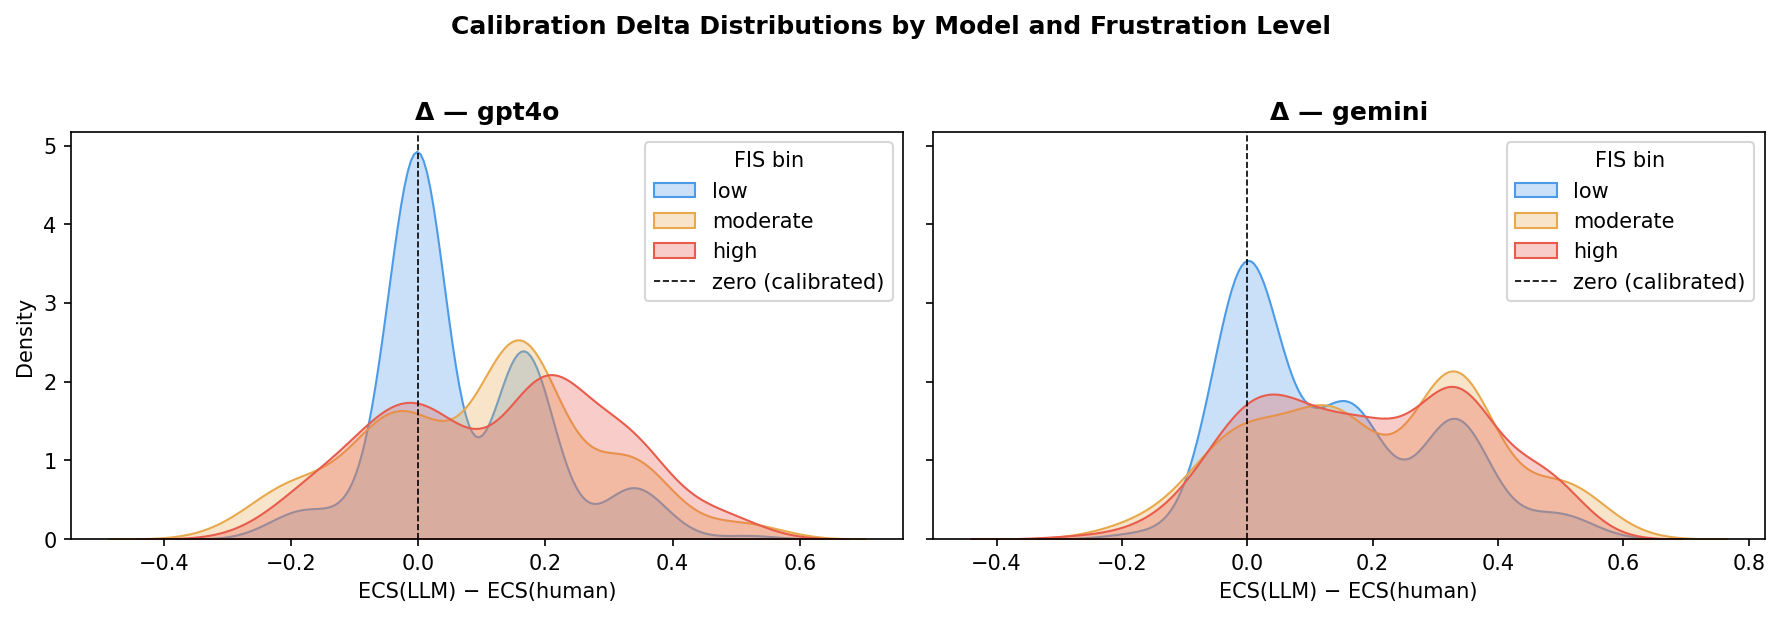
\includegraphics[width=\textwidth]{./delta_kde.png}
	\caption{Calibration Delta Distributions by Model and Frustration Level.}
	\label{fig:calibration delta}
\end{figure*}


\begin{figure*}[t]
	\centering
	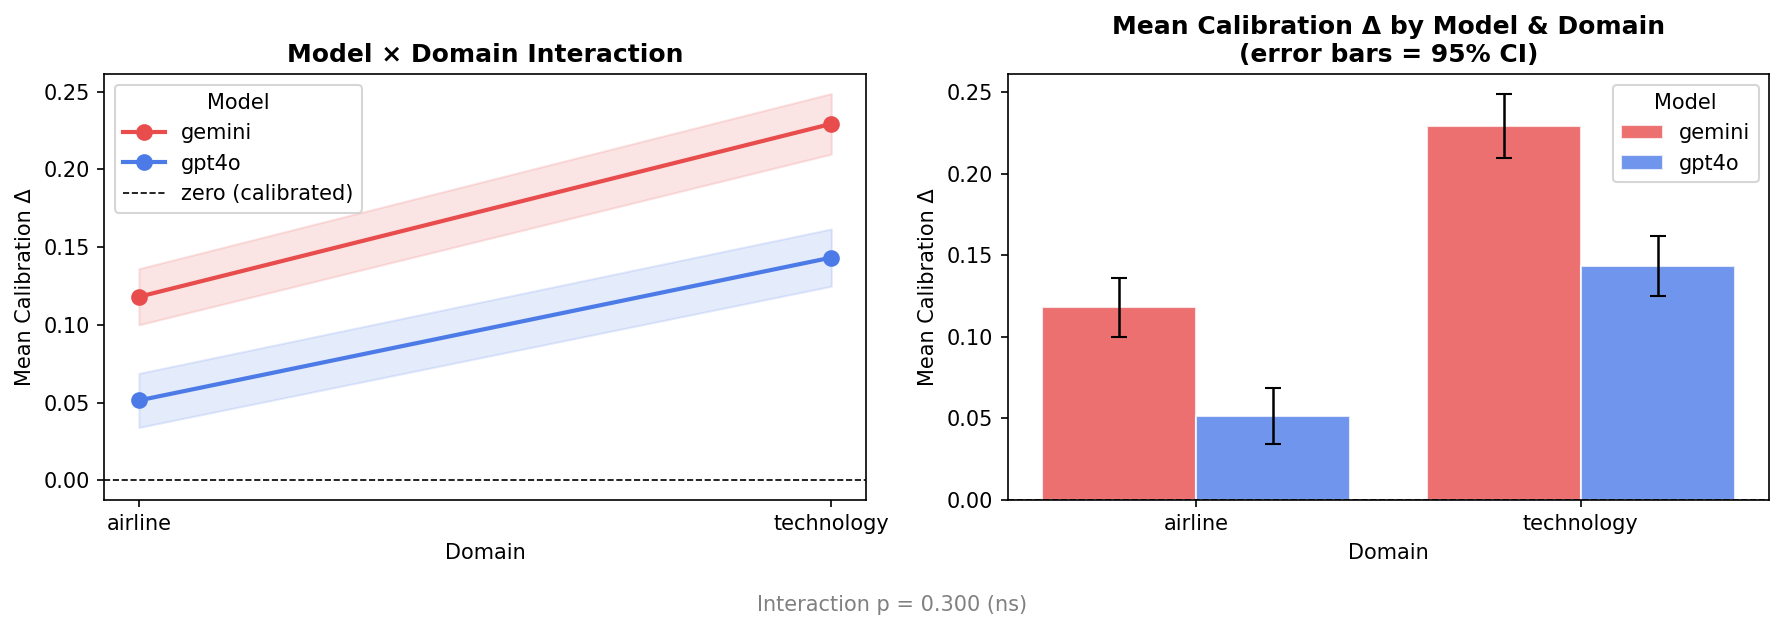
\includegraphics[width=\textwidth]{./anova_interaction.png}
	\caption{Model and Domain Relationship.}
	\label{fig:model and domain relation}
\end{figure*}


\subsection{Analysis}

Figure~\ref{fig:calibration delta} illustrates the distributions of calibration error ($\Delta$ = ECS\_{LLM} - ECS\_{human}) across different frustration levels for both GPT-4o and Gemini. A value of zero indicates perfect calibration, while positive values reflect systematic overestimation by the model.

For GPT-4o, the distribution under low frustration is sharply centered around zero, suggesting strong calibration when user frustration is minimal. However, as frustration increases, the distributions shift rightward and become more dispersed, indicating both increased overestimation and higher variance. This trend suggests that GPT-4o’s calibration degrades under more challenging emotional contexts.

In contrast, Gemini exhibits a consistent rightward shift across all frustration levels, with even low-frustration cases showing noticeable overestimation. The effect becomes more pronounced under moderate and high frustration, where the distributions are both further shifted and broader compared to GPT-4o. This indicates that Gemini not only overestimates more systematically but also demonstrates reduced stability.

Overall, both models are sensitive to user frustration, with higher frustration leading to greater positive calibration bias. However, GPT-4o remains better calibrated and more stable across conditions, whereas Gemini shows larger and more variable deviations from human judgments.

We also analyze model calibration across domains and examine whether domain-specific effects interact with model choice. Figure~\ref{fig:model and domain relation} summarizes the mean calibration error ($\Delta$) for two models across the airline and technology domains, with 95\% confidence intervals.

Across both domains, we observe a consistent gap between the two models: gpt4o exhibits lower calibration error than gemini. In the airline domain, gpt4o achieves a mean $\Delta$ of approximately 0.05, compared to 0.12 for gemini. This pattern persists in the technology domain, where gpt4o reaches ~0.14 while gemini increases to ~0.23. These results indicate that gpt4o is systematically better calibrated, regardless of domain.

In addition, both models show higher calibration error in the technology domain than in the airline domain. This suggests that the technology domain poses greater challenges for reliable confidence estimation, potentially due to increased ambiguity or broader knowledge requirements.


% ----------------------------------------------------------------------------------------


\section{Conclusions}

This work is designed to test how LLMs perform under different frustration level and whether LLMs will be over or under empathized and what is its driver. We answered the following question in this paper.

\begin{enumerate}
	\item \textbf{RQ1 — Do frontier LLMs systematically over- or under-empathize relative to human agents?}
	
	Both models show statistically significant positive calibration deltas, meaning both over-empathize relative to human agents. Also, there’s different tendency in models and frustration levels.
	
	
	\item \textbf{RQ2 — Is this miscalibration consistent across industry domains (airline vs. technology)?}
	
	The two-way ANOVA finds a significant main effect of domain, meaning both models over-empathize more in the technology sector than in the airline sector. A plausible interpretation: technology-sector human agents in the dataset tend to write more procedural, lower-warmth replies, so LLM defaults diverge more from that baseline than from the warmer airline-agent style.
	
\end{enumerate}

% ----------------------------------------------------------------------------------------

\section{Limitations}

Due to the token and API shortage, we limited our models on only GPT-4o and Gemini. More tested model would provide a better result and a more detailed explanation on whether the over-empathize is a universal problem or is it only related to these two models. 

Meanwhile, due to the limitation of customer service data, we cannot include all real-world conversation between a human agent and a customer. Thus, there might be a potential bias amount these analyzed data, which might cause the model to react over-empathized. 





% ----------------------------------------------------------------------------------------

\section{Challenges and Adjustments}

\subsection{Simplification from Original Design}

The original design included four ECS dimensions and a supervised fine-tuning (SFT) sub-experiment on Llama 3 8B as a contrastive model. Both were removed for scope and infrastructure reasons. The ECS was collapsed from four dimensions (apology density, urgency match, solution-orientation ratio, tone warmth) to two (apology density, tone-frustration fit). The two dropped dimensions---urgency match and solution ratio---are harder to define and score reliably in short tweets, and removing them produces a cleaner, more defensible metric. The SFT experiment requires GPU access, training pipelines, and at least two additional weeks, and is deferred to future work. The core empirical claim is fully supported without it.

\subsection{Model Availability}

Due to API access constraints during the experiment window, Claude 3.5 Sonnet could not be included in the main run. The pipeline is designed to append Claude responses and re-run scoring when access is restored; results in this report cover GPT-4o and Gemini 3 Flash only.

\bibliography{anthology,custom}
\bibliographystyle{acl_natbib}


% ----------------------------------------------------------------------------------------

\appendix

\section{Full Conversation Sample}
\label{Full-Conversation-Sample-twitter}
This section shows a sample of a full conversation.

\textbf{Customer:} @sprintcare I have sent several private messages and no one is responding as usual

\textbf{Sprintcare:} @115712 I understand. I would like to assist you. We would need to get you into a private secured link to further assist.

\textbf{Customer:} @sprintcare and how do you propose we do that

\textbf{Sprintcare:} @115712 Can you please send us a private message, so that I can gain further details about your account?

\textbf{Customer:} @sprintcare I did.

\textbf{Sprintcare:} @115712 Please send us a Private Message so that we can further assist you. Just click ‘Message’ at the top of your profile.

\textbf{Customer:} @sprintcare is the worst customer service

\end{document}